\documentclass[twoside]{scrreprt}

%Packages, die für die deutsch Sprache erforderlich sind
\usepackage[utf8]{inputenc}
\usepackage[T1]{fontenc}
\usepackage{lmodern}
\usepackage{ngerman}

%Packages für Graphik
\usepackage{graphicx}
\graphicspath{{Abbildungen/}}

%Package, damit Bibtex-URL klappt
\usepackage{url}

\begin{document}
%%%%% BEGINN TITELSEITE %%%%%
\begin{titlepage}

% Oberer Teil der Titelseite:
\begin{minipage}{0.4\textwidth}
	\begin{flushleft}
		\includegraphics[height=1.5cm]{TU_Logo}
	\end{flushleft}
\end{minipage}
\hfill
\begin{minipage}{0.4\textwidth}
	\begin{flushright}
		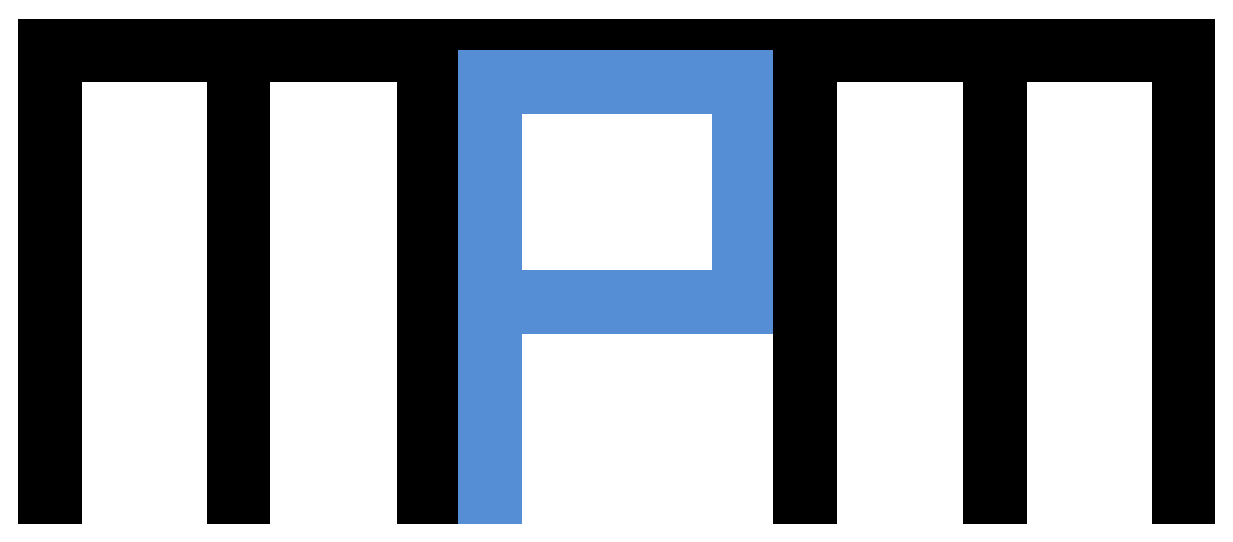
\includegraphics[height=1.5cm]{MPM_Logo}%TODO: Logo in HQ
	\end{flushright}
\end{minipage}

\begin{center}    
\textbf{\LARGE Technische Universität Berlin}\\
\large{Institut für Konstruktion, Mikro- und Medizintechnik}\\
\large{Fachgebiet Methoden der Produktentwicklung und Mechatronik}\\
\large{\textsc{Prof. Dr.-Ing. Dietmar Göhlich}}\\
\vfill

% Title
\huge{\textbf{Vergleich von Ladesystemen und Speichertechnologien für batteriebetriebene Stadtbusse}}\\
\rule{\linewidth}{1pt}
\large{Zur Erlangung des akademischen Grades Bachelor of Science}\\
\large{Im Studiengang Informationstechnik im Maschinenwesen}\\
\vfill

%Autor
\large{\textsc{Ludger Heide}}\\
\large{Matrikelnummer 338641}\\
\vfill

\large{Betreuerin: \textsc{M.Sc. Tu-Anh Ly}}\\
\vfill

\large{\today}
\end{center}
\end{titlepage}
%%%%% ENDE TITELSEITE %%%%%

\pagenumbering{Roman}
\chapter*{Abstract}
\addcontentsline{toc}{chapter}{Abstract}
\section*{English}
\section*{Deutsch}

\chapter*{Aufgabenstellung}
\addcontentsline{toc}{chapter}{Aufgabenstellung}

\chapter*{Eidesstattliche Erklärung}
\addcontentsline{toc}{chapter}{Eidesstattliche Erklärung}
Ich, Ludger Heide, versichere hiermit, dass ich meine Bachelorarbeit mit dem Thema
\begin{quote}
	\emph{Vergleich von Ladesystemen und Speichertechnologien für batteriebetriebene Stadtbusse}
\end{quote}
selbstständig verfasst und keine anderen als die angegebenen Quellen und Hilfsmittel benutzt habe, wobei ich alle wörtlichen und sinngemäßen Zitate als solche gekennzeichnet habe. Die Arbeit wurde bisher keiner anderen Prüfungsbehörde vorgelegt und auch nicht veröffentlicht.\\[6ex]
Berlin, \today\\
\newline
\rule{4cm}{0.5pt}\\
\textsc{Ludger Heide} 

\tableofcontents

\listoffigures
\addcontentsline{toc}{chapter}{Abbildungsverzeichnis}

\listoftables
\addcontentsline{toc}{chapter}{Tabellenverzeichnis}
\newpage

%%%%% BEGINN INHALT %%%%%
\pagenumbering{arabic}
\chapter{Einleitung}
\section{Kontext} %Namen ändern!
\subsection{Geschichte}
\subsection{Aktueller Stand}
\section{Problem} %TODO Namen ändern
\subsection{Ziel} %TODO: Nur im Text erwähnen?
\section{Methodik} %(Kurz))

\chapter{Ladesysteme} %Zewitens
\section{Bewertungskriterien} %TODO: Subsections
% Mit welcher Methode ausgewählt?
\section{Betrachtete Systeme} %TODO: Subsections
\section{Vergleichstabelle}

\chapter{Speichertechnologien} %Zuerst
Nach den Ladesystemen sollen hier nun die Speichertechnologien betrachtet werden. Sie lassen sich in mechanische, elektrische und elektrochemische Speicher aufteilen. In diesem Kapitel werden die Wirkprinzipien der in Bussen verwendeten Speichertechnologien erklärt.\\
\section{Mechanisch – Schwungradspeicher} %TODO: Quellen, warum endete die Gyrobuserprobung
Mechanische Energiespeicher für Fahrzeuge arbeiten mit komprimierter Luft oder Schwungrädern. Es gibt Prototypen reiner Pressluftantrieben in kleineren Fahrzeugen, in Bussen werden sie jedoch nur als Teil eines Hybridantriebs eingesetzt und hier nicht weiter betrachtet.\cite{Sebastian-Naumann:2014}. Im Schwungradspeicher wird die elektrische Energie in der Rotationsenergie eines Schwungrades gespeichert, das sich mit sehr hoher Geschwindigkeit dreht. Die Energieübertragung erfolgt durch eine elektrische Motor- und Generatoreinheit. Moderne Schwungräder werden aus gewickelten Karbonfasern hergestellt und in Vakuumgehäusen magnetisch gelagert. Im Falle eines berstenden Schwungrades muss das Gehäuse die gesamte Energie innerhalb von Sekundenbruchteilen aufnehmen, ohne selbst zu bersten. Dies erfordert sehr schwere Gehäuse, die die spezifische Energie und Leistung eines tatsächlichen Systems stark reduzieren. Der Schwungradspeicher wurde in den fünfziger Jahren im Gyrobus im schweizerischen Yverdon auf einer acht Kilometer langen Linie erprobt. Die acht Kilometer lange Strecke wurde erfolgreich zurückgelegt, die damalige Technologie war jedoch sehr wartungsaufwändig. Aktuell wird der Schwungradspeicher nur als Teil eines hybriden Antriebsstrangs eingesetzt.
\section{Elektrisch – Kondensator} %TODO: Quellen
Der Kondensator ist ein rein elektrischer Energiespeicher. Im klassischen Plattenkondensator werden zwei durch ein Dieelektrikum getrennte Platten elektrisch aufgeladen und die Ladung kann später wieder in Strom umgewandelt werden. Kondensatoren haben eine hohe spezifische Leistung, aber ihre spezifische Energie reicht nicht aus. In Bussen werden sogenannte Superkondensatoren verwendet, die statt eines festen Dieelektrikums eine polare Flüssigkeit verwenden und mithilfe des sogenannten Doppelschichteffektes und der Pseudokapazität weit höhere Energiedichten erreichn. In Shanghai werden Busse mit dieser Technologie seit 2008 im Linienverkehr eingesetzt.
\section{Chemisch}
\cite{Lajunen20141}
\section{Bewertungskriterien} %TODO: Subsections
\section{Betrachtete Systeme} %TODO: Subsections
\section{Vergleichstabelle}   %TODO: In den Anhang?

\chapter{Effizienzberechnung} %TODO: Besserer Titel %Drittens
\section{Ladesystem}
\section{Speichertechnologie}
\section{Ladestrategie und Route}
\section{Ergebnisse}
\subsection{Route A}
\subsection{Route B}

\chapter{Bewertung und Diskussion} %Diksussion
\section{Fazit}
\section{Ausblick}


%%%%% ENDE INHALT %%%%%

%Bibliographie
\bibliographystyle{alphadin}
\bibliography{Quellen/Quellenliste} 


\end{document}